\documentclass[abstracton,12pt]{scrartcl}
    
\usepackage[utf8]{inputenc}
% \usepackage[T1]{fontenc}
\usepackage{fancyhdr}
\usepackage{graphicx}
\usepackage{tikz}
\usepackage{listings}
\usepackage{amssymb}
\usepackage{amsfonts}
\usepackage{amsmath}
\usepackage{amsthm}
\usepackage{pdfpages}
\usepackage{forest}
\usepackage{multicol}
\usepackage{varwidth}
\usepackage{verbatim}
\usepackage{cleveref}
% \usepackage{minted}
\usepackage{framed}
\usepackage[ruled,vlined]{algorithm2e}
\usepackage{caption}
\usepackage{subcaption}
\usepackage{soul}
\usepackage{ulem}
\usepackage{ifthen}
% \usepackage{geometry}
% \usepackage{titlesec}

\forestset{qtree/.style={for tree={parent anchor=south, child anchor=north,align=left,inner sep=0pt}}}
\graphicspath{ {images/} }

% \setlength{\multicolsep}{6.0pt plus 2.0pt minus 1.5pt}% 50% of original values
% \titleformat{\chapter}{}{\thechapter}{}{}
% \titlespacing{\chapter}{-100pt}{-100pt}{-100pt}

% --------- 

\titlehead{Department of Informatics, University of Zürich}
\subject{\vspace*{2cm}MSc Basismodul}
\title{The Adaptive Radix Tree}
\author{
    Rafael Kallis\\[-5pt]
    \scriptsize Matrikelnummer: 14-708-887\\[-5pt]
    \scriptsize Email: \texttt{rk@rafaelkallis.com}
}
\date{\vspace*{2cm}September 1, 2018}
\publishers{
    \small supervised by Prof.\ Dr.\ Michael\ Böhlen and Kevin\ Wellenzohn \\[5cm]
    \begin{tikzpicture}[overlay]
    \node at (-3,-3) {
\includegraphics[height=1.5cm]{IFIlogo}};
    \node at (7,-3) {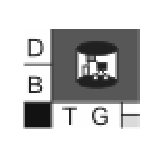
\includegraphics[height=1.5cm]{dbtgBW}};
    \end{tikzpicture}
}

% \dedication{dedicated to xxx}

% --------- 

\theoremstyle{definition}

\newtheorem{definition}{Definition}
% \newtheorem{figure}{Figure}
\newtheorem{example}{Example}
% \newtheorem{theorem}{Theorem}
% \newtheorem{lemma}{Lemma}

\crefname{algocfline}{algorithm}{algorithms}
\Crefname{algocfline}{Algorithm}{Algorithms}

\crefname{figure}{Fig.}{Figs.}
\Crefname{figure}{Figure}{Figures}

\crefname{example}{Ex.}{Ex.}
\Crefname{example}{Example}{Examples}

% \newenvironment{proof}
%     {\noindent{\bf Proof:\rm}}{\hfill$\Box$\vspace{\medskipamount}}

\newenvironment{centerverbatim}{\par\centering\varwidth{\linewidth}\verbatim}
    {\endverbatim\endvarwidth\par}

\def\bbbr{{\rm I\!R}}
\def\bbbm{{\rm I\!M}}
\def\bbbn{{\rm I\!N}}
\def\bbbz{{\rm I\!Z}}

% --------- 

\begin{document}

\maketitle

% \chapter*{Acknowledgements}

% \begin{abstract}
%   ...
% \end{abstract}

% \chapter*{Zusammenfassung}

% \tableofcontents
% \listoffigures
% \listoftables

\newpage
\section{Introduction}

Main-Memory Databases increasingly become a viable option for many applications.
Whilst main memory is a considerably faster medium than a secondary disk, 
utilizing caches more efficiently would lead to even better access times.

Leis et al.\ \cite{leis2013adaptive} propose the Adaptive Radix Tree (ART), an in-memory
data structure which efficiently stores and retrieves data, even outperforming
red-black trees.
As we will see later, ART achieves its exceptional performance, and space
efficiency, by compressing the tree both vertically and horizontally.
Higher space effiency allows ART to utilize caches more optimal.

The goal of this project is to implement ART, as proposed by 
\cite{leis2013adaptive} in C++ and compare its transactional throughput
against other in-memory data structures, i.e.\ red-black trees and hash tables.
In \Cref{sec:art} we describe how ART is constructed by applying 
vertical and horizontal compression to a trie.
Next, we describe the point and range query procedure, as well as 
value insertion and removal in \Cref{sec:operations}.
Finally, a benchmark of ART, a red-black tree and a hashtable
is presented in \Cref{sec:benchmarks}.

\section{Adaptive Radix Tree (ART)}
\label{sec:art}

The WAPI is a hierarchical index and indexes the properties of nodes.
It takes into account if an index node is volatile before performing structural index modifications.
If a node is considered volatile, we do not remove it from the index.
In the following section, we will see how to add, query and remove nodes from the index.

\subsection{Trie}

The trie \cite{fredkin1960trie} is a hierarchical data structure which
stores key-value pairs. The trie can answer both point and range queries 
efficiently since keys are stored sorted according to their lexicographic order.
A node's path represents the node's key. This is done by splitting a key into
chunks of $s$ bits, where $s$ is called \textit{span}. 

Each inner node has 
$2^s$ child nodes, one for each possible $s$-bit sequence. During tree
traversal, we propagate down to the child node identified by the $d$-th
$s$-bit chunk of the key, where $d$ is the depth of the current node. 
Using an array of $2^s$  pointers, this lookup can be done without any 
additional comparison. 

\Cref{fig:span} depicts tries storing the 
8-bit keys ``$01000011$'', ``$01000110$'' and ``$01100100$'' with 
$s=2, 4, 8$. Span $s$ is critical for the performance of the trie because $s$ 
determines the height of the trie. We observe that by increasing the span, 
we decrease the tree height. A trie
storing $k$ bit keys has $\lceil \frac{k}{s} \rceil$ levels of inner nodes.
As a consequence, point queries, insertions and deletions have 
$O(k)$ complexity. Having a data structure with
time complexity not dependend on $n$, makes it very attractive for large
data sets.

Span $s$ also determines the space consumption of the tree.
A node with span $s$ requires $2^s$ pointers. The tries in 
\Cref{fig:span} require a total of $240, 224, 384$ and $2048$ bytes 
respectively, for the bookeeping of child nodes, assuming 64-bit pointers.
An apparent trade off exists between tree height versus space efficiency that
depends on $s$.

\begin{figure}[h]
  \vspace{0mm}
  \begin{footnotesize}
    \begin{multicols}{3}
      \noindent
      \centering
      \framebox(140,160){
        \begin{forest}
          [,circle,draw
            [,circle,draw, edge label={node[midway,right,font=\footnotesize]{$01$}}
              [,circle,draw, edge label={node[midway,left,font=\footnotesize]{$00$}}
                [,circle,draw, edge label={node[midway,left,font=\footnotesize]{$00$}}
                  [,circle,draw, edge label={node[midway,left,font=\footnotesize]{$11$}}]
                ]
                [,phantom]
                [,circle,draw, edge label={node[midway,right,font=\footnotesize]{$01$}}
                  [,circle,draw, edge label={node[midway,right,font=\footnotesize]{$10$}}]
                ]
              ]
              [,phantom]
              [,phantom]
              [,circle,draw, edge label={node[midway,right,font=\footnotesize]{$10$}}
                [,circle,draw, edge label={node[midway,right,font=\footnotesize]{$01$}}
                  [,circle,draw, edge label={node[midway,right,font=\footnotesize]{$10$}}]
                ]
              ]
            ]
          ]
        \end{forest}
      }

      \vspace{2mm}
      \begin{normalsize}
        $s=2$
      \end{normalsize}
      \columnbreak
      ~

      \centering
      \framebox(140,160){
        \begin{forest}
          [,circle,draw
            [,circle,draw, edge label={node[midway,left,font=\footnotesize]{$0100$}}
              [,circle,draw, edge label={node[midway,left,font=\footnotesize]{$0011$}}]
              [,phantom]
              [,circle,draw, edge label={node[midway,right,font=\footnotesize]{$0110$}}]
            ]
            [,phantom]
            [,phantom]
            [,circle,draw, edge label={node[midway,right,font=\footnotesize]{$0110$}}
              [,circle,draw, edge label={node[midway,right,font=\footnotesize]{$0100$}}]
            ]
          ]
        \end{forest}
      }

      \vspace{2mm}
      \begin{normalsize}
        $s=4$
      \end{normalsize}
      \columnbreak
      ~

      \centering
      \framebox(140,160){
        \begin{forest}
          [,circle,draw
            [,circle,draw, edge label={node[midway,left,font=\scriptsize]{$01000011$}}]
            [,phantom]
            [,phantom]
            [,circle,draw, edge label={node[midway,font=\scriptsize]{$01000110$}}]
            [,phantom]
            [,phantom]
            [,circle,draw, edge label={node[midway,right,font=\scriptsize]{$01100100$}}]
          ]
        \end{forest}
      }

      \vspace{2mm}
      \begin{normalsize}
        $s=8$
      \end{normalsize}
      \columnbreak
      ~

    \end{multicols}
  \end{footnotesize}
  \caption{
    Tries with span $s=2,4,8$ storing keys ``$01000011$'', ``$01000110$''
    and ``$01100100$''.
  }
  \label{fig:span}
\end{figure}

\subsection{Vertical (Prefix) Compression}

When storing long keys, chains start to form where each node only has a
single child. As a consequence, we waste a lot of space on structural
information. Morrison introduced \textit{Patricia}~\cite{morrison1968patricia}. 
Patricia is a space-optimized trie in which
each node with no siblings is merged with its parent, i.e.\ inner nodes
are only created if they are required to distinguish at least two leaf nodes. 
Doing so, we eliminate chains caused by long keys which make tries 
space-inefficient. Although Morrison's Patricia tree is a bitwise trie, i.e.\ 
has a span $s=1$, the principle can be applied to tries with any span.
We refer to this heuristic as \textit{vertical compression}.

Vertical compression is implemented by storing an additional variable, called
\textit{prefix}, inside each node. This variable stores the concatenation
of partial keys of descendants that were eliminated because they had no 
siblings. \Cref{fig:vertical-compression} depicts two tries, one with and one 
without vertical compression. We observe that nodes with no siblings, color 
coded red, are eliminated and their partial key is appended to the parent's 
prefix. With even longer keys, the results of vertical compression are even 
more astonishing. 

Tall trees may become very compact, and so not only do we
save space that was otherwise wasted on structural inforation, we also are now
able to traverse the data structure even faster since the height decreased.

\begin{figure}[h]
  \begin{footnotesize}
    \begin{multicols}{2}
      \noindent
      \begin{flushright}
      \framebox(160,160){
        \begin{forest}
          [,circle,draw
            [,circle,draw,red, edge label={node[midway,right,font=\footnotesize]{$01$}}
              [,circle,draw, edge label={node[midway,left,font=\footnotesize]{$00$}}
                [,circle,draw, edge label={node[midway,left,font=\footnotesize]{$00$}}
                  [,circle,draw,red, edge label={node[midway,left,font=\footnotesize]{$11$}}]
                ]
                [,phantom]
                [,circle,draw, edge label={node[midway,right,font=\footnotesize]{$01$}}
                  [,circle,draw,red, edge label={node[midway,right,font=\footnotesize]{$10$}}]
                ]
              ]
              [,phantom]
              [,phantom]
              [,circle,draw, edge label={node[midway,right,font=\footnotesize]{$10$}}
                [,circle,draw,red, edge label={node[midway,right,font=\footnotesize]{$01$}}
                  [,circle,draw,red, edge label={node[midway,right,font=\footnotesize]{$10$}}]
                ]
              ]
            ]
          ]
        \end{forest}
      }
      \hspace{5mm}
      \end{flushright}
      ~

      \begin{flushleft}
      \hspace{5mm}
      \framebox(160,160){
        \begin{forest}
          [,circle,draw
            [,circle,draw, edge label={node[midway,left,font=\footnotesize]{$00$}}
              [,circle,draw, edge label={node[midway,left,font=\footnotesize]{$00$}}]{
                \draw[gray] (.east)--++(0.5em,0em)
                  node[anchor=west,gray]{11};
              }
              [,phantom]
              [,circle,draw, edge label={node[midway,right,font=\footnotesize]{$10$}}]{
                \draw[gray] (.east)--++(0.5em,0em)
                  node[anchor=west,gray]{01};
              }
            ]
            [,phantom]
            [,phantom]
            [,circle,draw, edge label={node[midway,right,font=\footnotesize]{$10$}}]{
              \draw[gray] (.east)--++(0.5em,0em)
                node[anchor=west,gray]{0110};
            }
          ]{
            \draw[gray] (.east)--++(0.5em,0em)
              node[anchor=west,gray]{01};
          }
        \end{forest}
      }
      \end{flushleft}
    \end{multicols}
  \end{footnotesize}
  \caption{
    Tries with span $s=2$ storing keys ``$01000011$'', ``$01000110$''
    and ``$01100100$''. The trie on the right incorporates vertical 
    compression. Red nodes indicate nodes which get eliminated under
    vertical compression. Gray strings represent the value of the ``prefix'' 
    property.
  }
  \label{fig:vertical-compression}
\end{figure}

\subsection{Horizontal Compression (Adaptive Nodes)}

With large values of span $s$, we sacrifice an excessive amount of space for a 
smaller tree height. Space is allocated for pointers which keep
references of child nodes. In order to reduce the space needed to keep
such references, Leis et al.\ propose \textit{Adaptive Nodes} 
\cite{leis2013adaptive}, which make use of dynamic data structures 
instead of static arrays for child node bookkeeping. Doing so, we allocate 
a minimal amount of space when the number of children is small and add more 
space if required, i.e.\ more children are added.
We refer to this heuristic as \textit{horizontal compression}.
Leis et al.\ also fix the span $s=8$, i.e. partial keys are 1 byte
long and therefore each node can have up to $2^8 = 256$ children.

An adaptive node is in one of four configurations, depending on the number
of children. Each of the four configurations is optimized for a different
number of children. The most compact configuration is called
\textit{Node4} which can carry up to four children. In the same manner,
we also have \textit{Node16}, \textit{Node48} and \textit{Node256}.

We now describe the structure of each of the four configurations.
The node types are also illustrated in \Cref{fig:horizontal-compression}.
We store the partial keys $65$, $82$, $84$ and their corresponding child nodes
$\alpha$, $\beta$, $\gamma$ in each node type with the purposes of explaining 
their structures. Note that $\emptyset$ is a \texttt{null} pointer.

A node of type Node4 contains two static arrays, each of which can hold
up to four values. The first array, called the ``partial keys'' array, holds
partial keys which identify children of that node. The second array,
called the ``children'' array, holds pointers to the child nodes.
Partial keys and pointers are stored at corresponding positions and
the partial keys are sorted. A node of type Node16 is structured similar
to Node4, the only difference being the lengths of the two static arrays,
which are now 16 each.

An instance of Node48 contains a 256-element array named 
``indexes'' and a 48-element array called ``children''.
Partial keys are stored implicitly in ``indexes'', i.e.\ 
can be indexed with partial key bytes directly.
As the name suggests, ``indexes'' stores the index of a child
node inside the ``children'' array. This node can be compared to
virtual memory, since the address space (256 addresses) is wider 
than the actual available storage space (48 slots).


\begin{figure}
  \vspace{-4cm}
  \hspace{-2cm}
  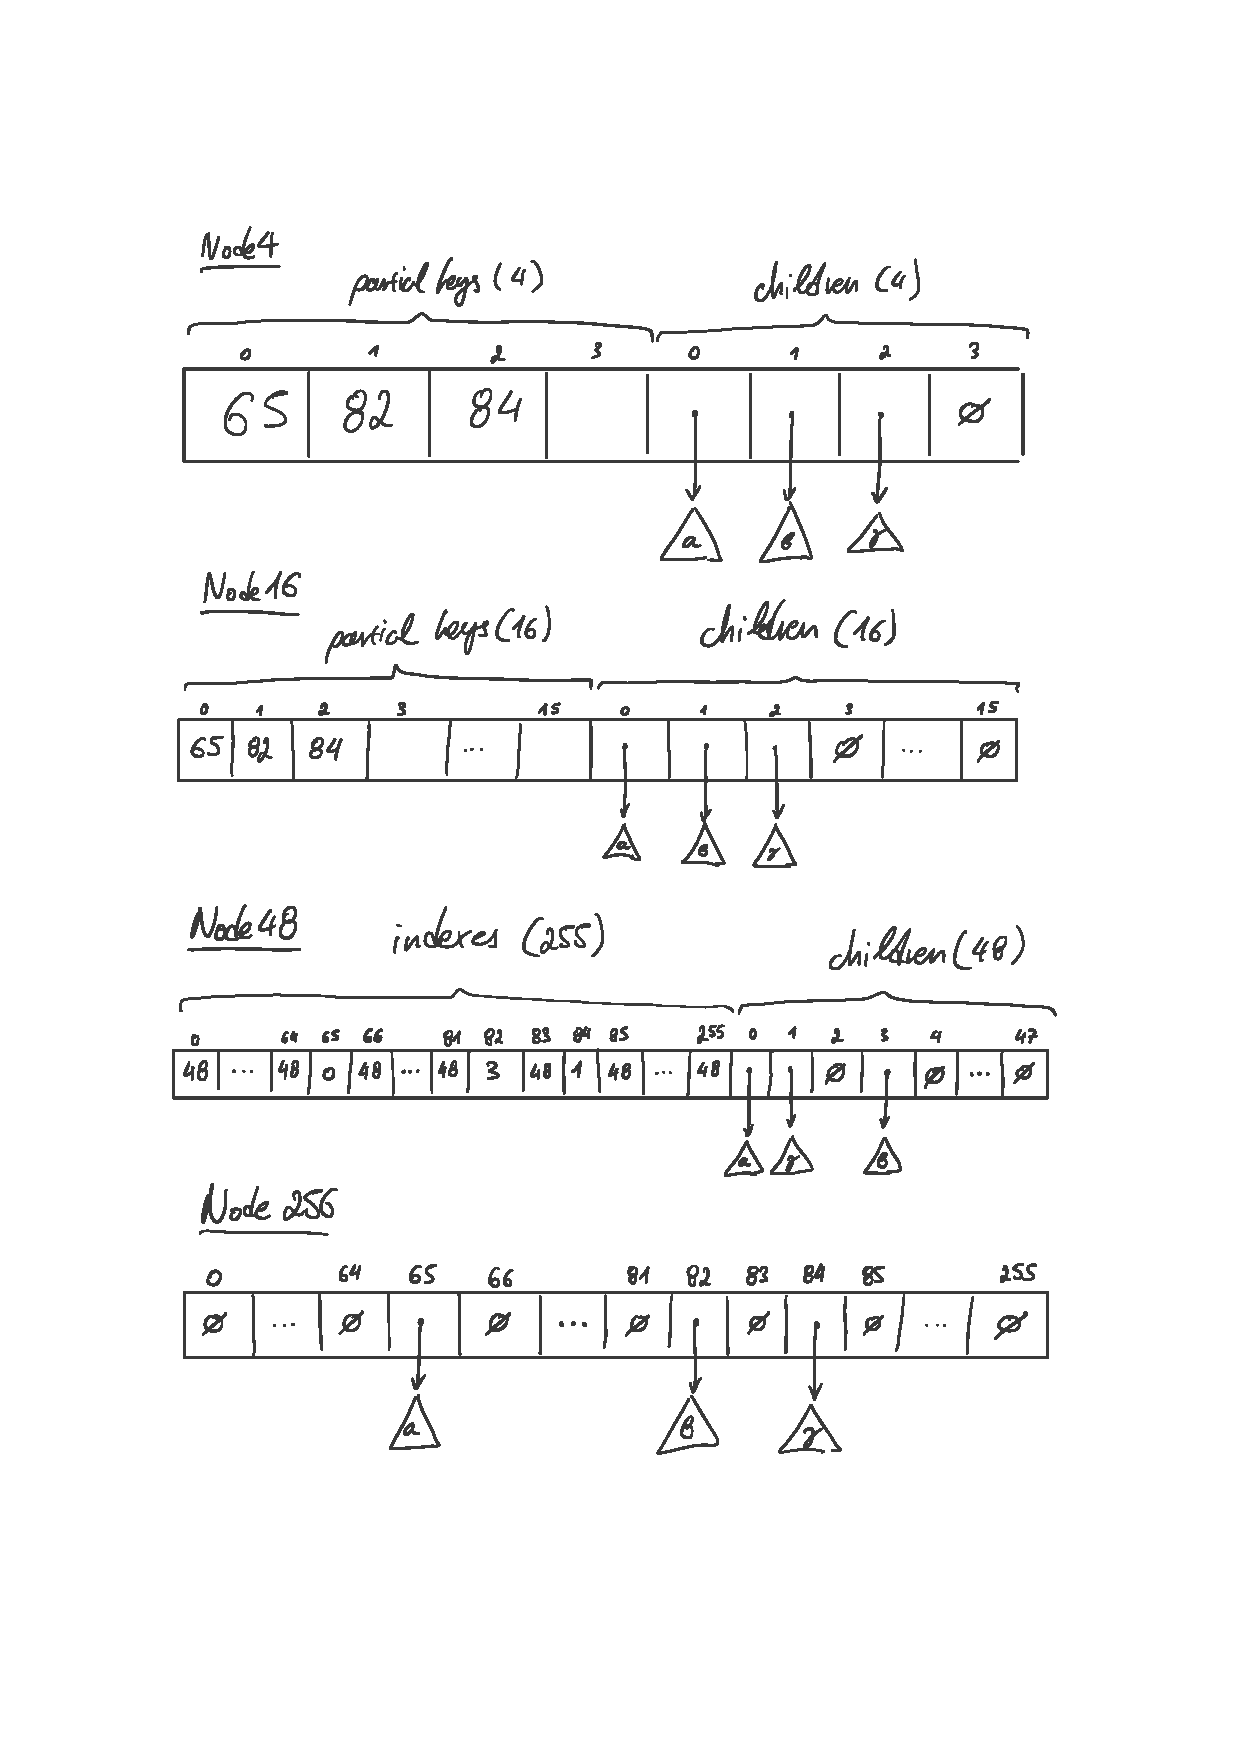
\includegraphics[height=27cm]{art_nodes_draw}
  \vspace{-3cm}
  \caption{
    Tries with span $s=2$ storing keys ``$01000011$'', ``$01000110$''
    and ``$01100100$''. The trie on the right incorporates vertical 
    compression. Red nodes indicate nodes which get eliminated under
    vertical compression. Gray strings represent the value of the ``prefix'' 
    property.
  }
  \label{fig:horizontal-compression}
\end{figure}

\newpage

\bibliographystyle{abbrv}
\bibliography{art}

\end{document}
